\chapter{Introduction}

\par
\hspace{1.2cm} Most of the systems using analog-to-digital converters (ADC's) bring signals with interesting statistical properties into operation, but Nyquist signal processing architectures do not take advantage of these properties. Actually, these signals (such as temperature sensors, pressure sensors, electro-cardiograms etc.) are almost always constant and may vary significantly only during brief moments like electrocardiograph as shown in Fig.~\ref{fig:ECG}. 

\begin{figure}[H]
	\begin{center}
		\includegraphics[scale=0.80]{./Figures/ECG.ps}
		\caption{Electrocardiograph (ECG) Signal.}
		\label{fig:ECG}
	\end{center}
\end{figure}

\par
\hspace{0.6cm} The classical regular sampling and converting systems are highly constrained, due to the Shannon theory, which is to ensure for the sampling frequency to be at least twice the maximum input signal frequency. Therefore, in the time domain, this condition can be translated as a large number of samples without any relevant information. This effect implies a useless increase of activity of the circuit compared to the supplied output digital information relevance, and so a useless increase of the power dissipation. It has been proved that ADC's using a non equi-repartition of the samples in time lead to interesting power savings compared to Nyquist ADC's~\cite{1522735}.



\section{Level cross sampling scheme}

\par
\hspace{0.6cm} The principle of level crossing ADC's is the dual case of Nyquist ADC's. In Nyquist \mbox{ADC's} the samples are taken at fixed intervals of time with reference to the clock signal. The minimum clock signal is chosen to be twice the maximum frequency of the analog input signal. For signals in which the frequency content is very low for most of the time, with rare occurrences of high frequency contents, it leads to over sampling. Hence, taking samples at regular intervals of time unnecessarily increases circuit activity, which in turn increases the power consumption~\cite{sayiner1996level}. 

\begin{figure}[H]
	\begin{center}
		\includegraphics[scale=0.75]{./Figures/LCS.ps}
		\caption{Principle of the level cross sampling scheme. }
		\label{fig:LCS}
	\end{center}
\end{figure}

\par
\hspace{1.2cm} In Nyquist ADC's the time instants are perfectly known and samples of amplitude are quantized, where as in case of level crossing ADC's the amplitude levels are known and the samples of time are quantized. Fig.~\ref{fig:LCS} shows the level cross sampling scheme~\cite{1595684}. In level crossing ADC's the occurrence of samples depend on signal amplitude variations, this sampling scheme removes the conversion of redundant samples or samples without any relevant information when the analog signal is quiet. Therefore, it leads to a compression of digital samples and reduction in the activity of the circuit. Level cross sampling is best suited for asynchronous and low power applications~\cite{allier2003new}. Difference between Nyquist sampling and level cross sampling schemes is illustrated in Table.~\ref{tab:DNL}. 

\begin{table}[H]
	\caption{Difference Between Nyquist \& Level Cross Sampling Schemes}
	\label{tab:DNL}
	\begin{center}
	\resizebox{10cm}{!}{
		\begin{tabular}{c|c|c|}
			\cline {2-3} %\hline
		 	&{Nyquist Sampling} & {Level Cross Sampling} \\ \hline
			\multicolumn {1}{|c|} {Conversion Trigger} 	&  {Clock} 			&  {Level Crossing} 	\\ \hline
			\multicolumn {1}{|c|} {Amplitude} 			&  {Quantized} 		&  {Exact Value} 		\\ \hline
			\multicolumn {1}{|c|} {Time} 				&  {Exact Value} 	&  {Quantized} 			\\ \hline
			\multicolumn {1}{|c|} {SNR Dependency} 		&  {Number of Bits} &  {Timer Period} 		\\ \hline
			\multicolumn {1}{|c|} {Converter Output} 	&  {Amplitude} 		&  {Amplitude \& Time} 	\\ \hline
		\end{tabular} }	
	\end{center}
\end{table}

\par
\hspace{0.6cm} In level crossing ADC's for M-bits resolution it requires $2^M-1$ quantization levels are regularly disposed along the amplitude range of the input signal $V_{in}$. A sample is taken only when the analog input signal $V_{in}$ crosses one of quantization levels. Contrary to classical Nyquist sampling, samples are not regularly spaced out in time, because it depends on the variation of input signal $V_{in}$~\cite{allier2005asynchronous}.

\begin{figure}[H]
	\begin{center}
		\includegraphics[height=10 cm, angle=270]{./Figures/ECGS.ps}
		\caption{Level cross sampling scheme for an ECG signal}
		\label{fig:ECGS}
	\end{center}
\end{figure}

\par
\hspace{0.6cm} 	The level cross sampling scheme can be understood by using Fig.~\ref{fig:ECGS}, which shows a typical ECG signal. Level crossing \mbox{ADC's} are driven by the level cross rather than by clock ie., the conversion process triggers when the analog input crosses any of the quantization levels. The dotted lines represent quantization levels. The shape of the analog input signal can be preserved by calculating the time difference between two successive samples. Thus, outputs from level crossing \mbox{ADC's} are amplitude and time data pairs, unlike that of Nyquist \mbox{ADC's} where the output consists of only amplitude data. 




\par
\hspace{0.6cm} The time taken from analog input crossing one of the quantization levels to complete conversion process is called loop delay of that level crossing ADC. The loop delay of the level crossing ADC's decides the maximum input signal frequency which can be track without slope overload error by the level crossing ADC. Fig.~\ref{fig:SOE} shows slope overloading error in level crossing ADC. The maximum frequency of the input with which the level crossing ADC can track without slope overload error can be calculated by using loop delay of the level crossing ADC~\cite{allier2005120nm}.



\par
\hspace{0.6cm} There are some drawbacks in level cross sampling ADC's, timer will define the resolution of the level crossing ADC's, which requires separate high speed clock generation circuit for timer to calculate the difference between present sample and previous sample. When tracking analog input signal it follows linear successive approximation which can't track sharp raise and fall edges in analog input signal~\cite{5672382}. When designing level crossing ADC's one must know the statistical properties of the signal clearly, once designed for particular application it can't be used for other application effectively. 

\begin{figure}[H]
	\begin{center}
		\includegraphics[scale=0.5]{./Figures/SOE.ps}
		\caption{Slope overloading error in LC-ADC}
		\label{fig:SOE}
	\end{center}
\end{figure}

\par
\hspace{0.6cm} The proposed architecture is aimed to reduce this loop delay so that it can track high frequency components in input analog signal without slope overloading error. It is achieved by reducing the conversion steps when the signal changes rapidly by checking for complete analog input range by incorporating binary search algoritham in conversion process.


\section{Organization of the Report}

\par
\hspace{1.2cm} The remainder of the report is organized as follows. Chapter 2 gives a brief overview on literature review of the level crossing ADC architectures. Chapter 3 describes the  proposed ADC architectures, its principle is based on a level cross sampling scheme that allow reduction in activity of the circuit. Chapter 4 presents building blocks and simulation results. Chapter 5 describes conclusion and future work.



